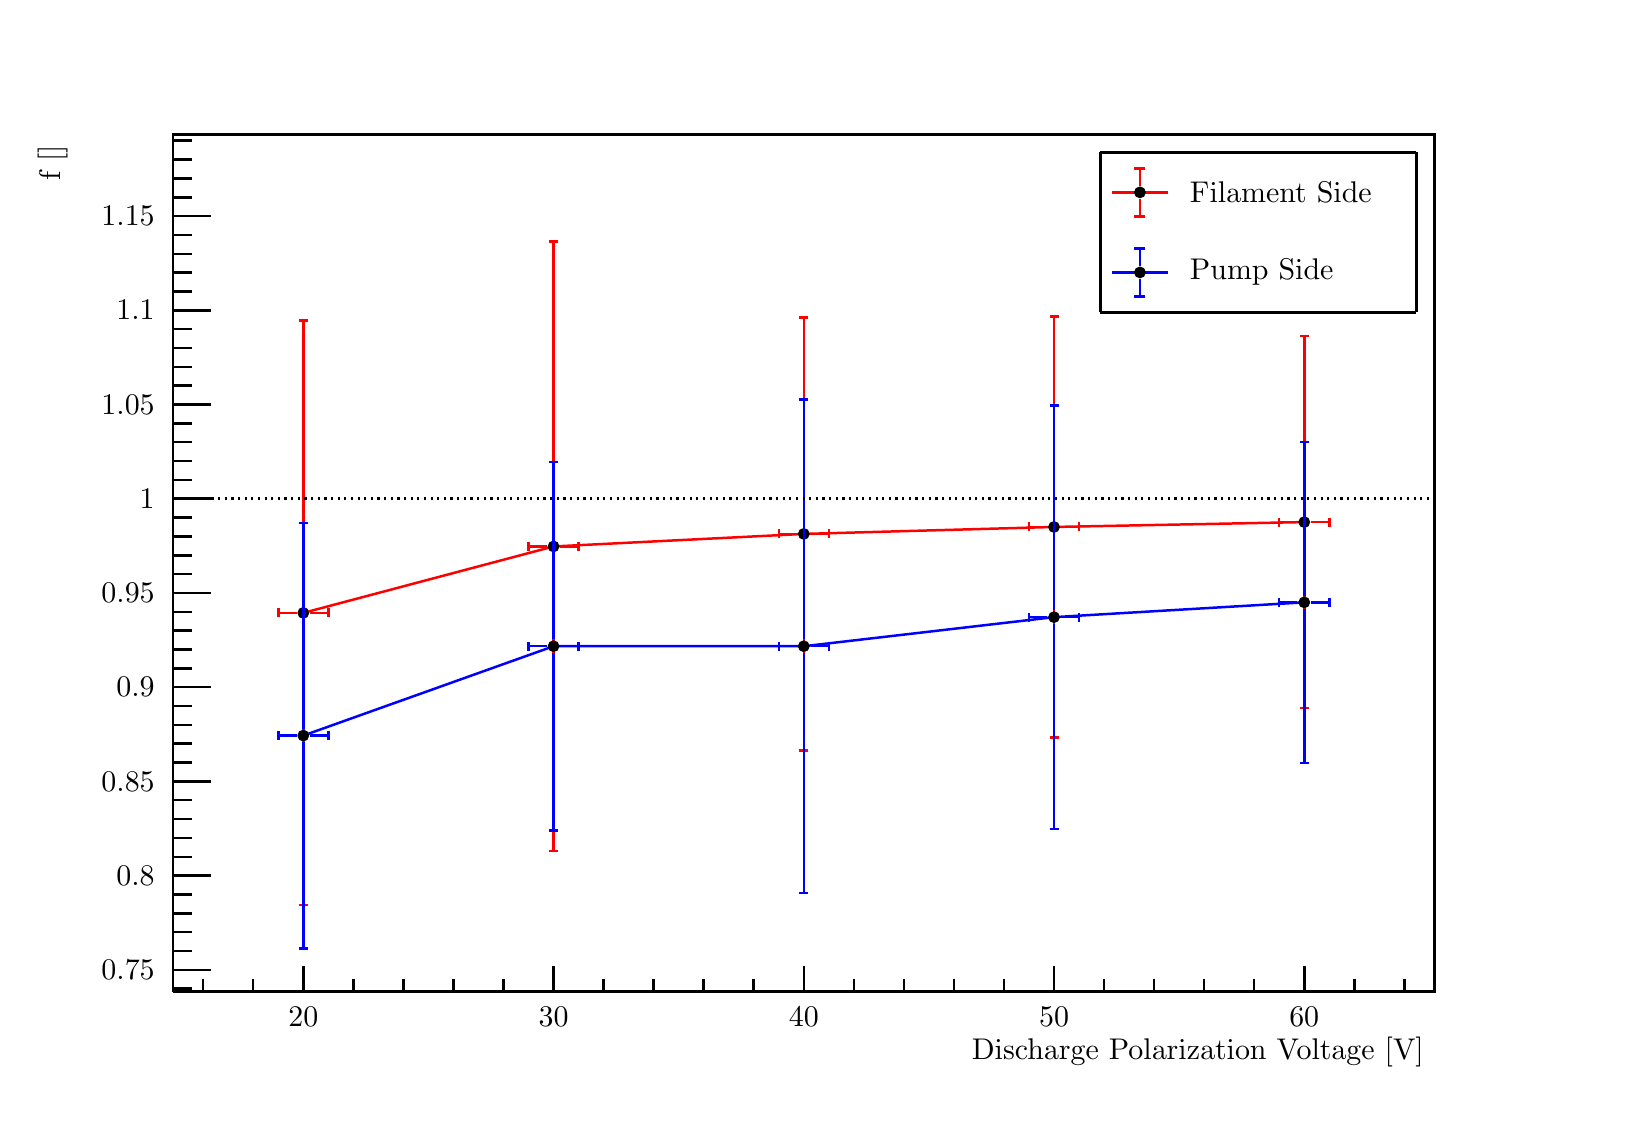
\begin{tikzpicture}
\pgfdeclareplotmark{cross} {
\pgfpathmoveto{\pgfpoint{-0.3\pgfplotmarksize}{\pgfplotmarksize}}
\pgfpathlineto{\pgfpoint{+0.3\pgfplotmarksize}{\pgfplotmarksize}}
\pgfpathlineto{\pgfpoint{+0.3\pgfplotmarksize}{0.3\pgfplotmarksize}}
\pgfpathlineto{\pgfpoint{+1\pgfplotmarksize}{0.3\pgfplotmarksize}}
\pgfpathlineto{\pgfpoint{+1\pgfplotmarksize}{-0.3\pgfplotmarksize}}
\pgfpathlineto{\pgfpoint{+0.3\pgfplotmarksize}{-0.3\pgfplotmarksize}}
\pgfpathlineto{\pgfpoint{+0.3\pgfplotmarksize}{-1.\pgfplotmarksize}}
\pgfpathlineto{\pgfpoint{-0.3\pgfplotmarksize}{-1.\pgfplotmarksize}}
\pgfpathlineto{\pgfpoint{-0.3\pgfplotmarksize}{-0.3\pgfplotmarksize}}
\pgfpathlineto{\pgfpoint{-1.\pgfplotmarksize}{-0.3\pgfplotmarksize}}
\pgfpathlineto{\pgfpoint{-1.\pgfplotmarksize}{0.3\pgfplotmarksize}}
\pgfpathlineto{\pgfpoint{-0.3\pgfplotmarksize}{0.3\pgfplotmarksize}}
\pgfpathclose
\pgfusepathqstroke
}
\pgfdeclareplotmark{cross*} {
\pgfpathmoveto{\pgfpoint{-0.3\pgfplotmarksize}{\pgfplotmarksize}}
\pgfpathlineto{\pgfpoint{+0.3\pgfplotmarksize}{\pgfplotmarksize}}
\pgfpathlineto{\pgfpoint{+0.3\pgfplotmarksize}{0.3\pgfplotmarksize}}
\pgfpathlineto{\pgfpoint{+1\pgfplotmarksize}{0.3\pgfplotmarksize}}
\pgfpathlineto{\pgfpoint{+1\pgfplotmarksize}{-0.3\pgfplotmarksize}}
\pgfpathlineto{\pgfpoint{+0.3\pgfplotmarksize}{-0.3\pgfplotmarksize}}
\pgfpathlineto{\pgfpoint{+0.3\pgfplotmarksize}{-1.\pgfplotmarksize}}
\pgfpathlineto{\pgfpoint{-0.3\pgfplotmarksize}{-1.\pgfplotmarksize}}
\pgfpathlineto{\pgfpoint{-0.3\pgfplotmarksize}{-0.3\pgfplotmarksize}}
\pgfpathlineto{\pgfpoint{-1.\pgfplotmarksize}{-0.3\pgfplotmarksize}}
\pgfpathlineto{\pgfpoint{-1.\pgfplotmarksize}{0.3\pgfplotmarksize}}
\pgfpathlineto{\pgfpoint{-0.3\pgfplotmarksize}{0.3\pgfplotmarksize}}
\pgfpathclose
\pgfusepathqfillstroke
}
\pgfdeclareplotmark{newstar} {
\pgfpathmoveto{\pgfqpoint{0pt}{\pgfplotmarksize}}
\pgfpathlineto{\pgfqpointpolar{44}{0.5\pgfplotmarksize}}
\pgfpathlineto{\pgfqpointpolar{18}{\pgfplotmarksize}}
\pgfpathlineto{\pgfqpointpolar{-20}{0.5\pgfplotmarksize}}
\pgfpathlineto{\pgfqpointpolar{-54}{\pgfplotmarksize}}
\pgfpathlineto{\pgfqpointpolar{-90}{0.5\pgfplotmarksize}}
\pgfpathlineto{\pgfqpointpolar{234}{\pgfplotmarksize}}
\pgfpathlineto{\pgfqpointpolar{198}{0.5\pgfplotmarksize}}
\pgfpathlineto{\pgfqpointpolar{162}{\pgfplotmarksize}}
\pgfpathlineto{\pgfqpointpolar{134}{0.5\pgfplotmarksize}}
\pgfpathclose
\pgfusepathqstroke
}
\pgfdeclareplotmark{newstar*} {
\pgfpathmoveto{\pgfqpoint{0pt}{\pgfplotmarksize}}
\pgfpathlineto{\pgfqpointpolar{44}{0.5\pgfplotmarksize}}
\pgfpathlineto{\pgfqpointpolar{18}{\pgfplotmarksize}}
\pgfpathlineto{\pgfqpointpolar{-20}{0.5\pgfplotmarksize}}
\pgfpathlineto{\pgfqpointpolar{-54}{\pgfplotmarksize}}
\pgfpathlineto{\pgfqpointpolar{-90}{0.5\pgfplotmarksize}}
\pgfpathlineto{\pgfqpointpolar{234}{\pgfplotmarksize}}
\pgfpathlineto{\pgfqpointpolar{198}{0.5\pgfplotmarksize}}
\pgfpathlineto{\pgfqpointpolar{162}{\pgfplotmarksize}}
\pgfpathlineto{\pgfqpointpolar{134}{0.5\pgfplotmarksize}}
\pgfpathclose
\pgfusepathqfillstroke
}
\definecolor{c}{rgb}{1,1,1};
\draw [color=c, fill=c] (0,0) rectangle (20,13.6103);
\draw [color=c, fill=c] (1.63324,1.37536) rectangle (17.6504,12.2636);
\definecolor{c}{rgb}{0,0,0};
\draw [c,line width=0.9] (1.63324,1.37536) -- (1.63324,12.2636) -- (17.6504,12.2636) -- (17.6504,1.37536) -- (1.63324,1.37536);
\definecolor{c}{rgb}{1,1,1};
\draw [color=c, fill=c] (1.63324,1.37536) rectangle (17.6504,12.2636);
\definecolor{c}{rgb}{0,0,0};
\draw [c,line width=0.9] (1.63324,1.37536) -- (1.63324,12.2636) -- (17.6504,12.2636) -- (17.6504,1.37536) -- (1.63324,1.37536);
\draw [c,line width=0.9] (1.63324,1.37536) -- (17.6504,1.37536);
\draw [c,line width=0.9] (3.28581,1.70236) -- (3.28581,1.37536);
\draw [c,line width=0.9] (3.92141,1.53886) -- (3.92141,1.37536);
\draw [c,line width=0.9] (4.55701,1.53886) -- (4.55701,1.37536);
\draw [c,line width=0.9] (5.19261,1.53886) -- (5.19261,1.37536);
\draw [c,line width=0.9] (5.82822,1.53886) -- (5.82822,1.37536);
\draw [c,line width=0.9] (6.46382,1.70236) -- (6.46382,1.37536);
\draw [c,line width=0.9] (7.09942,1.53886) -- (7.09942,1.37536);
\draw [c,line width=0.9] (7.73503,1.53886) -- (7.73503,1.37536);
\draw [c,line width=0.9] (8.37063,1.53886) -- (8.37063,1.37536);
\draw [c,line width=0.9] (9.00623,1.53886) -- (9.00623,1.37536);
\draw [c,line width=0.9] (9.64183,1.70236) -- (9.64183,1.37536);
\draw [c,line width=0.9] (10.2774,1.53886) -- (10.2774,1.37536);
\draw [c,line width=0.9] (10.913,1.53886) -- (10.913,1.37536);
\draw [c,line width=0.9] (11.5486,1.53886) -- (11.5486,1.37536);
\draw [c,line width=0.9] (12.1842,1.53886) -- (12.1842,1.37536);
\draw [c,line width=0.9] (12.8198,1.70236) -- (12.8198,1.37536);
\draw [c,line width=0.9] (13.4555,1.53886) -- (13.4555,1.37536);
\draw [c,line width=0.9] (14.0911,1.53886) -- (14.0911,1.37536);
\draw [c,line width=0.9] (14.7267,1.53886) -- (14.7267,1.37536);
\draw [c,line width=0.9] (15.3623,1.53886) -- (15.3623,1.37536);
\draw [c,line width=0.9] (15.9979,1.70236) -- (15.9979,1.37536);
\draw [c,line width=0.9] (3.28581,1.70236) -- (3.28581,1.37536);
\draw [c,line width=0.9] (2.6502,1.53886) -- (2.6502,1.37536);
\draw [c,line width=0.9] (2.0146,1.53886) -- (2.0146,1.37536);
\draw [c,line width=0.9] (15.9979,1.70236) -- (15.9979,1.37536);
\draw [c,line width=0.9] (16.6335,1.53886) -- (16.6335,1.37536);
\draw [c,line width=0.9] (17.2691,1.53886) -- (17.2691,1.37536);
\draw [anchor=base] (3.28581,0.926218) node[scale=1.08185, color=c, rotate=0]{20};
\draw [anchor=base] (6.46382,0.926218) node[scale=1.08185, color=c, rotate=0]{30};
\draw [anchor=base] (9.64183,0.926218) node[scale=1.08185, color=c, rotate=0]{40};
\draw [anchor=base] (12.8198,0.926218) node[scale=1.08185, color=c, rotate=0]{50};
\draw [anchor=base] (15.9979,0.926218) node[scale=1.08185, color=c, rotate=0]{60};
\draw [anchor= east] (17.6504,0.613181) node[scale=1.08185, color=c, rotate=0]{Discharge Polarization Voltage [V]};
\draw [c,line width=0.9] (1.63324,1.37536) -- (1.63324,12.2636);
\draw [c,line width=0.9] (2.11324,1.65229) -- (1.63324,1.65229);
\draw [c,line width=0.9] (1.87324,1.89159) -- (1.63324,1.89159);
\draw [c,line width=0.9] (1.87324,2.13089) -- (1.63324,2.13089);
\draw [c,line width=0.9] (1.87324,2.37019) -- (1.63324,2.37019);
\draw [c,line width=0.9] (1.87324,2.60949) -- (1.63324,2.60949);
\draw [c,line width=0.9] (2.11324,2.84879) -- (1.63324,2.84879);
\draw [c,line width=0.9] (1.87324,3.08809) -- (1.63324,3.08809);
\draw [c,line width=0.9] (1.87324,3.32738) -- (1.63324,3.32738);
\draw [c,line width=0.9] (1.87324,3.56668) -- (1.63324,3.56668);
\draw [c,line width=0.9] (1.87324,3.80598) -- (1.63324,3.80598);
\draw [c,line width=0.9] (2.11324,4.04528) -- (1.63324,4.04528);
\draw [c,line width=0.9] (1.87324,4.28458) -- (1.63324,4.28458);
\draw [c,line width=0.9] (1.87324,4.52388) -- (1.63324,4.52388);
\draw [c,line width=0.9] (1.87324,4.76318) -- (1.63324,4.76318);
\draw [c,line width=0.9] (1.87324,5.00248) -- (1.63324,5.00248);
\draw [c,line width=0.9] (2.11324,5.24178) -- (1.63324,5.24178);
\draw [c,line width=0.9] (1.87324,5.48108) -- (1.63324,5.48108);
\draw [c,line width=0.9] (1.87324,5.72037) -- (1.63324,5.72037);
\draw [c,line width=0.9] (1.87324,5.95967) -- (1.63324,5.95967);
\draw [c,line width=0.9] (1.87324,6.19897) -- (1.63324,6.19897);
\draw [c,line width=0.9] (2.11324,6.43827) -- (1.63324,6.43827);
\draw [c,line width=0.9] (1.87324,6.67757) -- (1.63324,6.67757);
\draw [c,line width=0.9] (1.87324,6.91687) -- (1.63324,6.91687);
\draw [c,line width=0.9] (1.87324,7.15617) -- (1.63324,7.15617);
\draw [c,line width=0.9] (1.87324,7.39547) -- (1.63324,7.39547);
\draw [c,line width=0.9] (2.11324,7.63477) -- (1.63324,7.63477);
\draw [c,line width=0.9] (1.87324,7.87406) -- (1.63324,7.87406);
\draw [c,line width=0.9] (1.87324,8.11336) -- (1.63324,8.11336);
\draw [c,line width=0.9] (1.87324,8.35266) -- (1.63324,8.35266);
\draw [c,line width=0.9] (1.87324,8.59196) -- (1.63324,8.59196);
\draw [c,line width=0.9] (2.11324,8.83126) -- (1.63324,8.83126);
\draw [c,line width=0.9] (1.87324,9.07056) -- (1.63324,9.07056);
\draw [c,line width=0.9] (1.87324,9.30986) -- (1.63324,9.30986);
\draw [c,line width=0.9] (1.87324,9.54916) -- (1.63324,9.54916);
\draw [c,line width=0.9] (1.87324,9.78846) -- (1.63324,9.78846);
\draw [c,line width=0.9] (2.11324,10.0278) -- (1.63324,10.0278);
\draw [c,line width=0.9] (1.87324,10.2671) -- (1.63324,10.2671);
\draw [c,line width=0.9] (1.87324,10.5064) -- (1.63324,10.5064);
\draw [c,line width=0.9] (1.87324,10.7457) -- (1.63324,10.7457);
\draw [c,line width=0.9] (1.87324,10.985) -- (1.63324,10.985);
\draw [c,line width=0.9] (2.11324,11.2242) -- (1.63324,11.2242);
\draw [c,line width=0.9] (2.11324,1.65229) -- (1.63324,1.65229);
\draw [c,line width=0.9] (1.87324,1.41299) -- (1.63324,1.41299);
\draw [c,line width=0.9] (2.11324,11.2242) -- (1.63324,11.2242);
\draw [c,line width=0.9] (1.87324,11.4635) -- (1.63324,11.4635);
\draw [c,line width=0.9] (1.87324,11.7028) -- (1.63324,11.7028);
\draw [c,line width=0.9] (1.87324,11.9421) -- (1.63324,11.9421);
\draw [c,line width=0.9] (1.87324,12.1814) -- (1.63324,12.1814);
\draw [anchor= east] (1.53324,1.65229) node[scale=1.08185, color=c, rotate=0]{0.75};
\draw [anchor= east] (1.53324,2.84879) node[scale=1.08185, color=c, rotate=0]{0.8};
\draw [anchor= east] (1.53324,4.04528) node[scale=1.08185, color=c, rotate=0]{0.85};
\draw [anchor= east] (1.53324,5.24178) node[scale=1.08185, color=c, rotate=0]{0.9};
\draw [anchor= east] (1.53324,6.43827) node[scale=1.08185, color=c, rotate=0]{0.95};
\draw [anchor= east] (1.53324,7.63477) node[scale=1.08185, color=c, rotate=0]{1};
\draw [anchor= east] (1.53324,8.83126) node[scale=1.08185, color=c, rotate=0]{1.05};
\draw [anchor= east] (1.53324,10.0278) node[scale=1.08185, color=c, rotate=0]{1.1};
\draw [anchor= east] (1.53324,11.2242) node[scale=1.08185, color=c, rotate=0]{1.15};
\draw [anchor= east] (0.102292,12.2636) node[scale=1.08185, color=c, rotate=90]{f []};
\definecolor{c}{rgb}{1,0,0};
\draw [c,line width=0.9] (3.28581,6.18475) -- (6.46382,7.02878) -- (9.64183,7.1879) -- (12.8198,7.27631) -- (15.9979,7.33815);
\definecolor{c}{rgb}{0,0,0};
\foreach \P in {(3.28581,6.18475), (6.46382,7.02878), (9.64183,7.1879), (12.8198,7.27631), (15.9979,7.33815)}{\draw[mark options={color=c,fill=c},mark size=1.921922pt,mark=*] plot coordinates {\P};}
\definecolor{c}{rgb}{1,0,0};
\draw [c,line width=0.9] (3.19985,6.18475) -- (2.968,6.18475);
\draw [c,line width=0.9] (2.968,6.12744) -- (2.968,6.24205);
\draw [c,line width=0.9] (3.37177,6.18475) -- (3.60361,6.18475);
\draw [c,line width=0.9] (3.60361,6.12744) -- (3.60361,6.24205);
\draw [c,line width=0.9] (3.28581,6.27071) -- (3.28581,9.89688);
\draw [c,line width=0.9] (3.2285,9.89688) -- (3.34311,9.89688);
\draw [c,line width=0.9] (3.28581,6.09879) -- (3.28581,2.47262);
\draw [c,line width=0.9] (3.2285,2.47262) -- (3.34311,2.47262);
\draw [c,line width=0.9] (6.37786,7.02878) -- (6.14602,7.02878);
\draw [c,line width=0.9] (6.14602,6.97147) -- (6.14602,7.08609);
\draw [c,line width=0.9] (6.54978,7.02878) -- (6.78162,7.02878);
\draw [c,line width=0.9] (6.78162,6.97147) -- (6.78162,7.08609);
\draw [c,line width=0.9] (6.46382,7.11474) -- (6.46382,10.8987);
\draw [c,line width=0.9] (6.40651,10.8987) -- (6.52113,10.8987);
\draw [c,line width=0.9] (6.46382,6.94282) -- (6.46382,3.15883);
\draw [c,line width=0.9] (6.40651,3.15883) -- (6.52113,3.15883);
\draw [c,line width=0.9] (9.55587,7.1879) -- (9.32403,7.1879);
\draw [c,line width=0.9] (9.32403,7.13059) -- (9.32403,7.2452);
\draw [c,line width=0.9] (9.72779,7.1879) -- (9.95963,7.1879);
\draw [c,line width=0.9] (9.95963,7.13059) -- (9.95963,7.2452);
\draw [c,line width=0.9] (9.64183,7.27386) -- (9.64183,9.93561);
\draw [c,line width=0.9] (9.58453,9.93561) -- (9.69914,9.93561);
\draw [c,line width=0.9] (9.64183,7.10194) -- (9.64183,4.44018);
\draw [c,line width=0.9] (9.58453,4.44018) -- (9.69914,4.44018);
\draw [c,line width=0.9] (12.7339,7.27631) -- (12.502,7.27631);
\draw [c,line width=0.9] (12.502,7.219) -- (12.502,7.33362);
\draw [c,line width=0.9] (12.9058,7.27631) -- (13.1376,7.27631);
\draw [c,line width=0.9] (13.1376,7.219) -- (13.1376,7.33362);
\draw [c,line width=0.9] (12.8198,7.36227) -- (12.8198,9.94895);
\draw [c,line width=0.9] (12.7625,9.94895) -- (12.8772,9.94895);
\draw [c,line width=0.9] (12.8198,7.19035) -- (12.8198,4.60368);
\draw [c,line width=0.9] (12.7625,4.60368) -- (12.8772,4.60368);
\draw [c,line width=0.9] (15.9119,7.33815) -- (15.6801,7.33815);
\draw [c,line width=0.9] (15.6801,7.28085) -- (15.6801,7.39546);
\draw [c,line width=0.9] (16.0838,7.33815) -- (16.3157,7.33815);
\draw [c,line width=0.9] (16.3157,7.28085) -- (16.3157,7.39546);
\draw [c,line width=0.9] (15.9979,7.42411) -- (15.9979,9.70058);
\draw [c,line width=0.9] (15.9406,9.70058) -- (16.0552,9.70058);
\draw [c,line width=0.9] (15.9979,7.25219) -- (15.9979,4.97573);
\draw [c,line width=0.9] (15.9406,4.97573) -- (16.0552,4.97573);
\definecolor{c}{rgb}{0,0,1};
\draw [c,line width=0.9] (3.19985,4.62693) -- (2.968,4.62693);
\draw [c,line width=0.9] (2.968,4.56962) -- (2.968,4.68423);
\draw [c,line width=0.9] (3.37177,4.62693) -- (3.60361,4.62693);
\draw [c,line width=0.9] (3.60361,4.56962) -- (3.60361,4.68423);
\draw [c,line width=0.9] (3.28581,4.71289) -- (3.28581,7.32944);
\draw [c,line width=0.9] (3.2285,7.32944) -- (3.34311,7.32944);
\draw [c,line width=0.9] (3.28581,4.54097) -- (3.28581,1.92442);
\draw [c,line width=0.9] (3.2285,1.92442) -- (3.34311,1.92442);
\draw [c,line width=0.9] (6.37786,5.76144) -- (6.14602,5.76144);
\draw [c,line width=0.9] (6.14602,5.70414) -- (6.14602,5.81875);
\draw [c,line width=0.9] (6.54978,5.76144) -- (6.78162,5.76144);
\draw [c,line width=0.9] (6.78162,5.70414) -- (6.78162,5.81875);
\draw [c,line width=0.9] (6.46382,5.8474) -- (6.46382,8.09901);
\draw [c,line width=0.9] (6.40651,8.09901) -- (6.52113,8.09901);
\draw [c,line width=0.9] (6.46382,5.67548) -- (6.46382,3.42388);
\draw [c,line width=0.9] (6.40651,3.42388) -- (6.52113,3.42388);
\draw [c,line width=0.9] (9.55587,5.76144) -- (9.32403,5.76144);
\draw [c,line width=0.9] (9.32403,5.70414) -- (9.32403,5.81875);
\draw [c,line width=0.9] (9.72779,5.76144) -- (9.95963,5.76144);
\draw [c,line width=0.9] (9.95963,5.70414) -- (9.95963,5.81875);
\draw [c,line width=0.9] (9.64183,5.8474) -- (9.64183,8.89504);
\draw [c,line width=0.9] (9.58453,8.89504) -- (9.69914,8.89504);
\draw [c,line width=0.9] (9.64183,5.67548) -- (9.64183,2.62784);
\draw [c,line width=0.9] (9.58453,2.62784) -- (9.69914,2.62784);
\draw [c,line width=0.9] (12.7339,6.13095) -- (12.502,6.13095);
\draw [c,line width=0.9] (12.502,6.07365) -- (12.502,6.18826);
\draw [c,line width=0.9] (12.9058,6.13095) -- (13.1376,6.13095);
\draw [c,line width=0.9] (13.1376,6.07365) -- (13.1376,6.18826);
\draw [c,line width=0.9] (12.8198,6.21691) -- (12.8198,8.82103);
\draw [c,line width=0.9] (12.7625,8.82103) -- (12.8772,8.82103);
\draw [c,line width=0.9] (12.8198,6.04499) -- (12.8198,3.44088);
\draw [c,line width=0.9] (12.7625,3.44088) -- (12.8772,3.44088);
\draw [c,line width=0.9] (15.9119,6.31887) -- (15.6801,6.31887);
\draw [c,line width=0.9] (15.6801,6.26156) -- (15.6801,6.37618);
\draw [c,line width=0.9] (16.0838,6.31887) -- (16.3157,6.31887);
\draw [c,line width=0.9] (16.3157,6.26156) -- (16.3157,6.37618);
\draw [c,line width=0.9] (15.9979,6.40483) -- (15.9979,8.35805);
\draw [c,line width=0.9] (15.9406,8.35805) -- (16.0552,8.35805);
\draw [c,line width=0.9] (15.9979,6.23291) -- (15.9979,4.27969);
\draw [c,line width=0.9] (15.9406,4.27969) -- (16.0552,4.27969);
\draw [c,line width=0.9] (3.28581,4.62693) -- (6.46382,5.76144) -- (9.64183,5.76144) -- (12.8198,6.13095) -- (15.9979,6.31887);
\definecolor{c}{rgb}{0,0,0};
\foreach \P in {(3.28581,4.62693), (6.46382,5.76144), (9.64183,5.76144), (12.8198,6.13095), (15.9979,6.31887)}{\draw[mark options={color=c,fill=c},mark size=1.921922pt,mark=*] plot coordinates {\P};}
\definecolor{c}{rgb}{1,1,1};
\draw [color=c, fill=c] (13.4097,10) rectangle (17.4212,12.0344);
\definecolor{c}{rgb}{0,0,0};
\draw [c,line width=0.9] (13.4097,10) -- (17.4212,10);
\draw [c,line width=0.9] (17.4212,10) -- (17.4212,12.0344);
\draw [c,line width=0.9] (17.4212,12.0344) -- (13.4097,12.0344);
\draw [c,line width=0.9] (13.4097,12.0344) -- (13.4097,10);
\draw [anchor= west] (14.4126,11.5258) node[scale=1.08185, color=c, rotate=0]{Filament Side};
\definecolor{c}{rgb}{1,0,0};
\draw [c,line width=0.9] (13.5602,11.5258) -- (14.2622,11.5258);
\draw [c,line width=0.9] (13.9112,11.6117) -- (13.9112,11.8309);
\draw [c,line width=0.9] (13.9112,11.4398) -- (13.9112,11.2206);
\draw [c,line width=0.9] (13.841,11.8309) -- (13.9814,11.8309);
\draw [c,line width=0.9] (13.841,11.2206) -- (13.9814,11.2206);
\definecolor{c}{rgb}{0,0,0};
\foreach \P in {(13.9112,11.5258)}{\draw[mark options={color=c,fill=c},mark size=1.921922pt,mark=*] plot coordinates {\P};}
\draw [anchor= west] (14.4126,10.5086) node[scale=1.08185, color=c, rotate=0]{Pump Side};
\definecolor{c}{rgb}{0,0,1};
\draw [c,line width=0.9] (13.5602,10.5086) -- (14.2622,10.5086);
\draw [c,line width=0.9] (13.9112,10.5946) -- (13.9112,10.8138);
\draw [c,line width=0.9] (13.9112,10.4226) -- (13.9112,10.2034);
\draw [c,line width=0.9] (13.841,10.8138) -- (13.9814,10.8138);
\draw [c,line width=0.9] (13.841,10.2034) -- (13.9814,10.2034);
\definecolor{c}{rgb}{0,0,0};
\foreach \P in {(13.9112,10.5086)}{\draw[mark options={color=c,fill=c},mark size=1.921922pt,mark=*] plot coordinates {\P};}
\draw [c,dash pattern=on 0.80pt off 1.60pt ,line width=0.9] (1.6968,7.63477) -- (17.6504,7.63477);
\end{tikzpicture}
